% Standalone copy of main.tex with tables/ and figures/ inlined; generated by paper/working_notes/verify/flatten.py.
% Edit main.tex (the modular source) or this file, but not both.
% Working Notes: team carnot, FinReason Cup 2026 Task 1.
% Organiser format: IEEE two-column conference template, at most 10 pages INCLUDING references,
% single-blind (author names and affiliations visible). See paper/ORGANISER_REQUIREMENTS.md.
% Every number in this file is traced to its source in paper/VERIFICATION.md.
\documentclass[conference]{IEEEtran}
\usepackage[T1]{fontenc}
\usepackage[utf8]{inputenc}
\usepackage{amsmath}
\usepackage{booktabs}
\usepackage{graphicx}
\usepackage[hyphens]{url}
\usepackage{tikz}
\usetikzlibrary{arrows.meta,positioning,calc}
\usepackage[hidelinks]{hyperref}
\hypersetup{pdftitle={Exact Program-of-Thought with Pre-Registered Evaluation for Verifiable Financial Chain Reasoning: Team carnot at FinReason Cup 2026 Task 1}, pdfauthor={Joel Jobi}}
\newcommand{\id}[1]{\texttt{#1}}
% Public repository (given by the author on 18 November 2026).
\newcommand{\repourl}{https://github.com/joelynx/IEEE-carnot}

\begin{document}

\title{Exact Program-of-Thought with Pre-Registered Evaluation for Verifiable Financial Chain Reasoning:\\ Team carnot at FinReason Cup 2026 Task~1}

% Single author (confirmed by the author on 15 October 2026). Remove the e-mail line if it should not be shown.
\author{\IEEEauthorblockN{Joel Jobi}
\IEEEauthorblockA{\textit{Indian Institute of Technology Delhi -- Abu Dhabi}\\
Abu Dhabi, United Arab Emirates\\
24a1cseb0013@iitdabudhabi.ac.ae}}

\maketitle

\begin{abstract}
Team carnot's system for Task~1 of the FinReason Cup 2026 answers template-generated financial questions with a final answer and named intermediate values; templates that were never released carry half of the test score. A language model writes one short Python program per question, a sandbox executes it with exact rational arithmetic, a formatter renders each field from its published specification, and the organisers' validator checks each row; questions without a train counterpart are answered by a five-sample per-field vote. On the development leaderboard the final system, R4, scores 1.000000 on final answers and 0.999167 on reasoning steps, against 0.984444 and 0.990000 for the strongest organiser baseline. The residual errors we inspected were misread slot conventions. On familiar templates, a run without the worked examples lost two final answers in 580, and the five-sample vote returned the answers of its first sample. Changes aimed at the hidden templates were pre-registered and screened on fixed splits with a lockbox; these screens could detect harm on familiar templates but could not measure hidden-template gains, and our synthetic hidden-like sets were too easy to separate systems. In the official results R4 ranks 17th of 27 teams, with combined final-answer correctness 0.985304 and hidden-stratum correctness 0.976025. The published scores imply three wrong final answers among 580 seen-template questions and eight among 348 hidden-template questions; the hidden questions are longer and more conditional than the released ones, and the samples disagree on them more often. Code, prompts, logs and the response cache are public.
\end{abstract}

\begin{IEEEkeywords}
financial reasoning, program of thought, exact arithmetic, self-consistency, pre-registered evaluation, shared task
\end{IEEEkeywords}

\section{Introduction}
Task~1 of the FinReason Cup 2026~\cite{finreason2026overview,finreason2026task1overview} asks a system to answer template-generated financial calculation questions and to expose its intermediate values. Each question publishes a specification of the final answer (a unit and a rounding rule, or an enumeration of allowed strings) and an ordered list of named intermediate \emph{slots}, each with a one-sentence description and its own specification. A prediction is scored by exact match on two measures: final-answer correctness (FAC) and a checkpoint score, the share of a question's slots whose value matches the reference. The test set has two strata. The \emph{seen} stratum comes from the 290 templates for which labelled data were released; the \emph{hidden} stratum comes from templates that were never released. The two strata are weighted equally in the ranking, and hidden FAC is the first tie-breaker. The task builds on FinChain~\cite{xie-etal-2026-finchain}, a symbolic benchmark of parameterised financial templates with executable solutions over the same 12 domains and 58 topics. The organisers describe FinChain as a provenance and novelty reference only; we did not use it in the system (Section~\ref{sec:integrity}).

Two properties of the task shaped the design. First, scoring is exact: a half-up field is compared after quantisation to the published places, an exact field is compared as a rational number, and one malformed value invalidates the whole file, so arithmetic and formatting errors cost as much as reasoning errors. We therefore execute programs with exact rational arithmetic and render each field from its published specification. Transcendental functions and root-finding remain finite-precision approximations, which are allowed only in half-up fields (Section~\ref{sec:sandbox}). Neither measure checks that a program computes the right quantity. Second, the residual errors we inspected concern the organisers' conventions, for example whether an ``annual compound multiplier'' covers one year or the whole horizon. Such conventions can be learned for seen templates and are unknown for hidden ones.

Program-of-thought prompting and self-consistency are established methods, and we propose no new prompting technique. What we add is an implementation in which the executed value is the submitted value, an audited evaluation record, and negative results:
\begin{enumerate}
\item a pipeline whose final system, R4, scores 1.000000 (final answer) and 0.999167 (reasoning steps) on the development leaderboard, above the organisers' published baselines (Sections~\ref{sec:system} and~\ref{sec:results});
\item an error and component analysis on labelled data: the residual errors are misread conventions, a stronger model fixed one convention but broke other slots, borrowing conventions from other templates failed because slot names are not used consistently, and on familiar templates the five-sample vote returned the answers of its first sample (Sections~\ref{sec:components}, \ref{sec:negative} and~\ref{sec:errors});
\item an evaluation design with fixed splits, a lockbox, paired bootstrap comparisons and pre-registration, together with its limit: it can detect harm on familiar templates but cannot measure hidden-template gains (Sections~\ref{sec:method} and~\ref{sec:post});
\item replayable submissions and a public record: the R3 and R4 test submissions regenerate byte-identically from the released response cache, and decisions, disclosures and incidents are logged (Section~\ref{sec:integrity}).
\end{enumerate}
The official test results place R4 17th of 27 teams with a hidden-stratum FAC of 0.976025 (Section~\ref{sec:test}). Our development checks did not anticipate this gap; Section~\ref{sec:hidden} sets out what the public record shows about it.

\paragraph*{Related work}
Program-aided and program-of-thought prompting~\cite{gao2023palprogramaidedlanguagemodels,chen2023programthoughtspromptingdisentangling} separate reasoning from computation by having the model write code that an interpreter runs; we add exact rational arithmetic and rendering from the published specification, so that the executed program's value is the submitted value. Chain-of-thought prompting~\cite{NEURIPS2022_9d560961} and self-consistency decoding~\cite{wang2023selfconsistencyimproveschainthought} motivate the sampled programs and the plurality vote on the novel route. Earlier financial numerical-reasoning benchmarks such as FinQA~\cite{chen-etal-2021-finqa}, TAT-QA~\cite{zhu-etal-2021-tat} and ConvFinQA~\cite{chen-etal-2022-convfinqa} score final answers over tables and text; FinChain~\cite{xie-etal-2026-finchain} and this task also score the intermediate chain, which is where our residual errors lie.

\section{Task, Data and Scoring}\label{sec:task}

\subsection{Records and rendering conventions}
A question record holds the question text, an \id{answer\_spec} and a \id{trace\_spec}. The text ends with a generated ``Answer format'' sentence. A decimal specification names a unit from a fixed set and a rounding mode, either \emph{exact} or \emph{half-up} to a given number of places; an enum specification lists the allowed strings. The trace specification is an ordered list of slots, each with a \id{slot\_id}, a free-text description and its own specification. Gold values are strings: half-up values are padded to the published places; exact values are a minimal decimal when the denominator divides a power of ten and otherwise an irreducible fraction such as \id{3/11}; enums are case-sensitive. Percent-type units are in percentage points (a premium of 6 percent is \id{6}), whereas ratios are plain fractions.

\subsection{Data}
We use the FinReason Cup 2026 Task~1 release, \url{https://the-finai.github.io/IEEE-bigdata-cup/task1/}, licensed under CC BY 4.0 (\url{https://creativecommons.org/licenses/by/4.0/}); we made no changes to the data. The development data contract is \id{task1-v4} and the test release is \id{task1-v4-test-questions-20260901-r2}; every file was hash-checked against its release manifest on every run. The release has 2,900 train questions (ten per template), 290 development questions (one per template), 580 development-leaderboard questions without gold and 928 test questions without gold. The 290 seen templates span 58 topics in 12 domains, with 116 basic, 116 intermediate and 58 advanced templates. Train final answers are 2,700 decimals and 200 enums; train questions carry 5,180 slot instances (320 questions have no slot, 690 have one, 1,180 two and 710 three). Train and development together hold 8,888 gold fields: 3,091 half-up, 5,379 exact and 418 enum. The test file has 1,492 slots over 928 questions, 64 of which have no slot.

\subsection{Scoring and ranking}
Scores come from the organisers' frozen scorer, version \id{finreason.task1.scorer/2.0.0} at toolkit commit \id{983537c}, which they confirmed is the test scorer. It matches each field exactly: enum strings must be equal; exact decimals are compared as rational numbers; half-up decimals are quantised to the published places with round-half-up on both sides and then compared. A case scores FAC~$=1$ if its final answer matches. Its checkpoint score is the number of matching slots divided by the number of published slots; cases without slots are excluded from the checkpoint metric. Scores aggregate hierarchically: the mean over the cases of a template, the mean over templates within a (domain, topic, difficulty) cell, a difficulty-weighted mean per topic (seen weights basic 2/5, intermediate 2/5, advanced 1/5; hidden weights 1/2 and 1/2), the mean over topics per domain, and the mean over the 12 domains. We give official scores to six decimal places, as the organisers do. A file with one invalid row (an unknown slot, a duplicate, an out-of-order step, a malformed decimal or an enum outside the vocabulary) is rejected as a whole. The organisers confirmed that the final ranking is the descending lexicographic order of (combined FAC, hidden FAC, combined checkpoint), each key quantised to six decimal places with round-half-even, where ``combined'' is the equal-weighted mean of the seen and hidden strata; ties share a rank.

\subsection{Seen and hidden strata}\label{sec:strata}
The scorer's frozen counts give 580 seen and 348 hidden test questions. A rule built from train alone (Section~\ref{sec:routing}) flags exactly 348 test questions as novel and none of the train, development, lockbox or leaderboard questions; each of the 290 released templates matches exactly two of the other 580. We assume, but cannot verify, that the 348 are the hidden questions; we call them the \emph{novel route} and the other 580 the \emph{seen route}. Their public fields differ markedly from train (Section~\ref{sec:hidden}). No labelled example of a hidden template exists, so the hidden stratum, half of the combined score and the first tie-breaker, cannot be measured with released data.

\section{System}\label{sec:system}
% ---- begin figures/pipeline.tex (inlined) ----
% Pipeline figure (DOSSIER §3.1). Pure TikZ; no external file.
\begin{figure}[t]
\centering
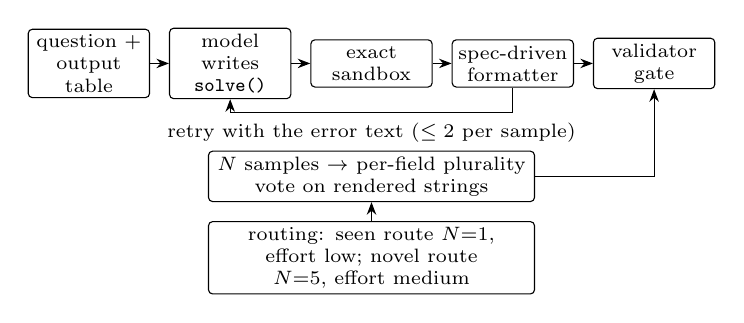
\begin{tikzpicture}[
  font=\scriptsize,
  box/.style={draw, rounded corners=1.5pt, align=center, inner sep=2pt, minimum height=6mm, text width=14mm},
  arr/.style={-{Stealth[length=1.6mm]}},
  node distance=2.4mm
]
\node[box] (q) {question $+$\\output table};
\node[box, right=of q] (m) {model writes\\\texttt{solve()}};
\node[box, right=of m] (s) {exact\\sandbox};
\node[box, right=of s] (f) {spec-driven\\formatter};
\node[box, right=of f] (g) {validator\\gate};
\draw[arr] (q) -- (m);
\draw[arr] (m) -- (s);
\draw[arr] (s) -- (f);
\draw[arr] (f) -- (g);
\draw[arr] (f.south) -- ++(0,-3.2mm) -| node[pos=0.25, below] {retry with the error text ($\le 2$ per sample)} (m.south);
\node[box, text width=40mm, below=8mm of s] (v) {$N$ samples $\to$ per-field plurality vote on rendered strings};
\node[box, text width=40mm, below=2.4mm of v] (r) {routing: seen route $N{=}1$, effort low; novel route $N{=}5$, effort medium};
\draw[arr] (r) -- (v);
\draw[arr] (v.east) -| ($(g.south)+(0,-1.5mm)$) -- (g.south);
\end{tikzpicture}
\caption{The pipeline for one question; Section~\ref{sec:system} gives the details. A field that is still invalid after the retries is omitted.}
\label{fig:pipeline}
\end{figure}
% ---- end figures/pipeline.tex ----
% ---- begin tables/systems.tex (inlined) ----
% T-D: the submitted systems (DOSSIER §3.7; facts.json#runs.*.routing, configs/r0..r4.json)
\begin{table}[t]
\caption{The systems. Sonnet = \texttt{claude-sonnet-5-5}, Opus = \texttt{claude-opus-5-5}; $N$ = samples per question with a per-field plurality vote.}
\label{tab:systems}
\centering
\scriptsize
\setlength{\tabcolsep}{4pt}
\begin{tabular}{@{}lp{2.0cm}p{2.55cm}p{1.55cm}@{}}
\toprule
System & Seen route & Novel route & Test status \\
\midrule
R0 & Sonnet, effort low, $N{=}1$ & no routing; as seen & accepted \\
R1 & $=$ R0 & Sonnet, effort medium, $N{=}5$ & accepted \\
R2 & $=$ R0 & Opus, effort medium, $N{=}5$ & packaged, not uploaded \\
R3 & $=$ R0 & $=$ R1 $+$ unit hint v2 & accepted \\
R4 & R0 $+$ unit hint v2 $+$ echo notes & $=$ R3 $+$ echo notes (never fire on test) & accepted, latest \\
\bottomrule
\end{tabular}
\end{table}
% ---- end tables/systems.tex ----

\subsection{Pipeline}
For every question the solver builds a prompt (Fig.~\ref{fig:pipeline}) from a fixed system prompt (the rules of the sandbox, the unit conventions and the instruction to follow the question's own definitions and scenario-local rules), three worked examples (Section~\ref{sec:exemplars}), the question verbatim, and a table of required outputs: the key \id{final} and every slot id, each with its description and a short rendering of its specification (for example ``number in percent, percentage points (5.25 means 5.25\,\%); checked as an exact value (return it unrounded)''). The model answers with one Python code block defining \id{solve()}, which returns a dictionary with exactly those keys.

The sandbox executes the program and the formatter renders each value from its specification; when execution fails, a key is missing or a value cannot be rendered, up to two retries per sample re-prompt with the failing program and the error text. With $N>1$ samples a per-field plurality vote selects the rendered strings (Section~\ref{sec:voting}). Each row then passes the toolkit's \id{validate\_prediction\_record} before it is written. A field that is still invalid is omitted rather than edited (a final becomes \id{null}), which costs only that field; this fallback was declared in advance, and no run needed it: every test submission has a non-null final for all 928 questions and all 1,492 slots. Submissions are produced with the toolkit's own \id{validate}, \id{package} and \id{validate-zip} commands.

\subsection{Verified worked examples}\label{sec:exemplars}
The three worked examples are fixed and were chosen mechanically. Three categories are defined from public specification fields only: (A) a decimal final with at least two exact slots including a percent or ratio unit; (B) an enum final with at least one decimal slot; (C) a decimal final with at least one half-up slot. For each category, templates of the exemplar pool (a subset of the tuning split, Section~\ref{sec:splits}) are visited in a seeded order and one case per template is solved zero-shot by the base solver; a program is kept only if the official scorer gives a correct final and every slot correct against train gold. Two verified programs per category, from distinct templates, are kept as a primary and a backup; all six were verified at the first attempt (WACC, early-retirement bridge and bond coupon reinvestment as primaries; VaR time horizon, disclosure threshold and after-tax net sale cost as backups). Every prompt shows the three primaries; in leave-template-out evaluation a backup replaces a primary that shares the question's template. There is no retrieval, so same-template examples are never shown.

\subsection{Exact-arithmetic sandbox}\label{sec:sandbox}
Programs run under a code policy and an arithmetic rewrite. An AST whitelist admits imports of \id{math}, \id{fractions}, \id{decimal}, \id{itertools}, \id{functools} and a helper module, and rejects classes, \id{with} blocks, \id{eval}, \id{exec}, \id{open}, dunder names and private attributes. The AST is then rewritten so that every float literal becomes an exact rational (\id{0.05} becomes \id{Q("0.05")}) and every arithmetic operator becomes an exact helper; division of integers is exact and \id{float()} raises. The helper module provides \id{sqrt}, \id{ln}, \id{exp}, \id{erf}, the standard normal CDF, bisection root-finding and half-up rounding. Only rational operations are exact: irrational results, and anything computed from them, are 60-digit decimals, and bisection stops at a tolerance of $10^{-45}$ unless the program sets another; the formatter accepts such values only in half-up fields. Programs execute in a WSL2 Ubuntu guest inside \id{unshare -rmn} (new user, mount and network namespaces; no network; Windows drives hidden behind a tmpfs), one child process per program with resource limits and a five-second timeout.

\subsection{Spec-driven formatter and validator gate}
The formatter receives each returned value and emits the submitted string; no other component writes a value. An exact field becomes a minimal finite decimal when the denominator is of the form $2^a5^b$ and otherwise an irreducible \id{n/d}; a half-up field is quantised with round-half-up to the published places and padded; an enum is checked for membership. In an exact field an inexact value (a float or a 60-digit decimal) is a rendering error that triggers a retry; a half-up field rounds it, and a float is flagged in the log. A round-trip test checks the rendering itself: it re-renders all 8,888 gold values of train and development and requires byte equality, and it passes. Since the formatter is the only writer and the validator checks every row, each submitted string is the rendered value of an executed program.

\subsection{Self-consistency}\label{sec:voting}
With $N$ samples the solver takes, for each field independently, the plurality of the rendered strings over the samples that rendered that field. The equivalence is the scorer's own (identical rendering at the published places), so no tolerance is added. A tie goes to the string held by the sample that agrees with the per-field plurality on the most fields, then to the lowest sample index. A field with no valid candidate is omitted. Fields are voted independently, so each field comes from an executed program but a row may combine several programs; the validator checks each field's format and does not check relations between slots.

\subsection{Routing rule}\label{sec:routing}
Rule \id{novel\_vs\_train\_v1} declares a question novel if neither its number-masked text skeleton (lower-cased, whitespace-normalised, the ``Answer format'' sentence removed, every number replaced by \id{\#}) nor its ordered list of (slot id, description) pairs occurs among the 2,900 train questions. The rule is fixed, derived from train and uses only these public fields. It sends 348 test questions, and no train, development, lockbox, tuning-eval or leaderboard question, to the novel route.

\subsection{Model access and reproducibility}\label{sec:model}
All model calls go to Claude models through the Claude Code command-line interface (version 2.1.296) in headless mode on a Claude subscription: one subprocess per call with our own system prompt, no tools, a single turn and JSON output, from an empty working directory with a scrubbed environment. The interface exposes no temperature or seed, so samples are independent calls, and reproducibility comes from a response cache keyed by model, effort, interface version, flag version, the hashes of the system and user prompts, the sample index and the attempt tag. Every replay we checked reproduced its run bit for bit (Section~\ref{sec:integrity}). The returned model identifier was recorded for every call; across all 69,277 cached calls, including the post-submission experiments and the ablation of Section~\ref{sec:components}, it equals the requested identifier.

\subsection{The submitted systems}\label{sec:systems}
Table~\ref{tab:systems} defines the systems R0 to R4; R1 introduces the routing rule. Two prompt changes need detail. \emph{Unit hint v2} (R3 on the novel route, R4 on both routes) describes a \id{dimensionless} field in the required-outputs table as ``a pure number with no unit; keep the scale of the question's own quantities (do not rescale percentages to fractions unless the description says so)'' instead of ``a plain number (0.0525, not 5.25)''. \emph{Echo notes} (R4, both routes): when a sentence of the question repeats a slot description verbatim (after lower-casing, whitespace normalisation and dropping the final period), the required-outputs table states that the sentence belongs to that slot and is not the definition of the final answer. The echo trigger fires on none of the 348 novel-route test questions, so R4's novel-route answers are R3's. The system prompt was not changed and still says that outputs in ratio, multiple or dimensionless units are plain numbers; the more specific per-field hint changed the behaviour.

\section{Evaluation Methodology}\label{sec:method}

\subsection{Splits, lockbox and modes}\label{sec:splits}
Train and development, eleven labelled cases per template, were split once with a recorded seed. The \emph{lockbox} (all 290 development cases plus two train cases per template, 870 cases) is reserved for confirming candidates: four logged looks were allowed and two were used, and after the first, in which three cases were inspected (Section~\ref{sec:errors}), results were read as aggregates only. The \emph{tuning} split holds the other eight train cases per template (2,320). Of these, \emph{tuning-eval} is two fixed cases per template (580), the \emph{exemplar pool} is the rest (1,740) and the only source of worked examples, and \emph{tuning-noex} is tuning minus the six exemplar cases (2,314). Every template appears in every split. The development leaderboard was used twice: as a pipeline check for R0 and as the decisive check for R4.

Labelled evaluations run in two modes. S-mode uses the fixed examples as deployed; H-mode excludes examples from the question's own template. Because the system has no retrieval, H-mode changes the worked examples of only 6 of 580 tuning-eval and 21 of 2,314 tuning-noex questions and otherwise differs in the resampling unit, so agreement between the modes is a sensitivity check and not an independent replication.

\subsection{Comparisons and decision rules}\label{sec:compare}
Labelled runs are scored with the toolkit's \id{score\_submission}. For a comparison, per-case weights are obtained from the scorer by one-hot probing, each run's score is recomputed from them and checked against the toolkit's report, and the difference (candidate minus baseline) is bootstrapped with shared resample indices (10,000 replicates, fixed seed; cases within templates in S-mode, templates within topics in H-mode). Run-to-run noise was measured with three R0 runs on tuning-eval with fresh samples (FAC 1.000000, 0.998333 and 1.000000), which gives $\sigma_{\mathrm{run}}(\mathrm{FAC})=0.000962$ and $\sigma_{\mathrm{run}}(\mathrm{checkpoint})=0.000481$. Three runs of one configuration give only a rough noise scale, and every threshold below inherits that uncertainty.

Two rules were fixed before any candidate was run. The \emph{improvement rule} adopts a candidate if the paired 95\,\% interval of $\Delta$ excludes 0, $\Delta>2\sigma_{\mathrm{run}}$, and one subsequent lockbox look gives $\Delta>0$. Changes aimed at the hidden stratum fall under the \emph{adoption rule} (recorded in the pre-registration as a non-inferiority rule). The change is pre-registered with its configuration and code hashes and its pass and fail actions before any of its outputs exist; it acts only through the train-derived routing rule; forced onto every tuning-eval question in both modes, neither score is detectably lower ($\Delta\ge-2\sigma_{\mathrm{run}}$ and an interval whose upper bound is $\ge0$, four of four); and no statistic computed on test outputs is used. The author approved each candidate's specification before it was built, and every pre-registration, result and incident is logged.

The adoption rule tests only for detectable degradation, with a point-estimate tolerance, and does not establish statistical non-inferiority: an interval that contains 0 can also contain substantial harm (R2's H-mode checkpoint interval reaches $-0.006667$). Adoption under it rests on prior evidence and the absence of detected harm on familiar templates. The supplementary material (Section~\ref{sec:integrity}) gives the full protocol.

\section{Results}\label{sec:results}
% ---- begin tables/labelled.tex (inlined) ----
% T-A: results on labelled data (TABLES.md T2; facts.json#runs; DOSSIER §5.1). Official toolkit scores, seen stratum, 6 dp.
\begin{table}[t]
\caption{Official scores on labelled data (seen stratum; 6 decimal places). ``Forced'' applies the novel-route configuration to every question. Lockbox rows are aggregates only.}
\label{tab:labelled}
\centering
\scriptsize
\begin{tabular}{@{}llrr@{}}
\toprule
System & Split ($n$), mode & FAC & Checkpoint \\
\midrule
R0 & tuning-eval (580), S and H & 1.000000 & 0.995675 \\
R0 & lockbox (870), S (look 1) & 0.996667 & 0.996508 \\
R0 & tuning-noex (2,314), S & 0.999167 & 0.997192 \\
R1 forced & tuning-eval, S and H & 1.000000 & 0.996508 \\
R2 forced & tuning-eval, S and H & 1.000000 & 0.995556 \\
R3 forced & tuning-eval, S and H & 1.000000 & 0.997619 \\
R4 forced & tuning-eval, S and H & 1.000000 & 0.997619 \\
R4 seen route & tuning-noex (2,314), S & 1.000000 & 0.998304 \\
\midrule
e\_base & tuning-noex, H & 0.998750 & 0.997282 \\
e\_conv & tuning-noex, H & 0.997917 & 0.996726 \\
e\_hint & tuning-noex, H & 0.998750 & 0.998601 \\
e\_base & lockbox (870), H (look 2) & 0.995556 & 0.996508 \\
e\_hint & lockbox (870), H (look 2) & 0.995556 & 0.997063 \\
\bottomrule
\end{tabular}
\end{table}
% ---- end tables/labelled.tex ----
% ---- begin tables/baselines.tex (inlined) ----
% T-B: development leaderboard vs organiser baselines (TABLES.md T5; facts.json#organiser, #submissions.development_portal_responses)
\begin{table}[t]
\caption{Development leaderboard (580 questions): organiser baselines by their published labels and our two uploads.}
\label{tab:baselines}
\centering
\scriptsize
\begin{tabular}{@{}lrr@{}}
\toprule
System & Final answer & Reasoning steps \\
\midrule
Lite (organiser baseline) & 0.234048 & 0.555354 \\
Standard (organiser baseline) & 0.980556 & 0.987725 \\
Advanced (organiser baseline) & 0.984444 & 0.990000 \\
carnot R0 ($=$ R1 $=$ R3 on this set) & 0.998333 & 0.998056 \\
carnot R4 (final) & \textbf{1.000000} & \textbf{0.999167} \\
\bottomrule
\end{tabular}
\end{table}
% ---- end tables/baselines.tex ----
% ---- begin tables/decisions.tex (inlined) ----
% T-C: pre-registered decisions (TABLES.md T3; facts.json#comparisons; experiments/preregistration.jsonl)
\begin{table*}[t]
\caption{Pre-registered comparisons: $\Delta$ is candidate minus baseline on the official seen scores, as an exact fraction, with the paired-bootstrap 95\,\% interval of Section~\ref{sec:compare}. ``Forced'' applies the novel-route configuration to every tuning-eval question.}
\label{tab:decisions}
\centering
\scriptsize
\setlength{\tabcolsep}{3pt}
\begin{tabular}{@{}llllp{5.4cm}@{}}
\toprule
Candidate vs.\ baseline & Set, mode & $\Delta$FAC [95\,\% CI] & $\Delta$checkpoint [95\,\% CI] & Rule; decision \\
\midrule
R1 forced vs.\ R0 & tuning-eval, S & 0 [0, 0] & $+1/1200$ [0, $+0.001667$] & adoption rule; pass 4/4, R1 adopted \\
 & tuning-eval, H & 0 [0, 0] & $+1/1200$ [0, $+0.002500$] & \\
R2 forced vs.\ R1 forced & tuning-eval, S & 0 [0, 0] & $-1/1050$ [$-0.002619$, $+0.000714$] & adoption rule; pass 4/4 against the limit $-0.000962$, not uploaded \\
 & tuning-eval, H & 0 [0, 0] & $-1/1050$ [$-0.006667$, $+0.004762$] & \\
conventions\_v1 vs.\ e\_base & tuning-noex, H & $-1/1200$ [$-0.002500$, 0] & $-1/1800$ [$-0.004821$, $+0.003056$] & improvement; rejected, R1 stays \\
hints\_v2 vs.\ e\_base & tuning-noex, H & 0 [0, 0] & $+19/14400$ [0, $+0.003542$] & breakage check; pass (9 changed, all fixes) \\
 & lockbox, H (look 2) & 0 [0, 0] & $+1/1800$ [$-0.001111$, $+0.002778$] & $\Delta>0$ and FAC not detectably lower; pass (direction only), build R3 \\
R3 forced vs.\ R1 forced & tuning-eval, S & 0 [0, 0] & $+1/900$ [$+0.001111$, $+0.001111$] & adoption rule; pass 4/4, R3 adopted \\
 & tuning-eval, H & 0 [0, 0] & $+1/900$ [0, $+0.003333$] & \\
R4 seen route vs.\ R0 & tuning-noex, S & $+1/1200$ [0, $+0.002083$] & $+1/900$ [$+0.000486$, $+0.001736$] & safety check; pass (finals 2 fixed, 0 broken; slots 9 fixed, 1 broken; biased, see text) \\
R4 forced vs.\ R3 forced & tuning-eval, S and H & 0 [0, 0] & 0 [0, 0] & adoption rule; identical, 0 changed cases \\
R4 routed vs.\ R0 & dev leaderboard & 0.998333 $\to$ 1.000000 & 0.998056 $\to$ 0.999167 & no drop and one rise; pass, R4 adopted and uploaded \\
\bottomrule
\end{tabular}
\end{table*}
% ---- end tables/decisions.tex ----

\subsection{Labelled data}
R0 answers every tuning-eval question correctly in both modes and misses five slots; on the lockbox it has three wrong finals in 870 cases (Table~\ref{tab:labelled}). Forcing the novel-route configuration onto every tuning-eval question leaves FAC at 1.000000 for R1, R2, R3 and R4. On the larger tuning-noex set the R4 seen route reaches FAC 1.000000 and checkpoint 0.998304, against 0.999167 and 0.997192 for R0.

\subsection{Development leaderboard}
Both of our development uploads score above the organisers' baselines (Table~\ref{tab:baselines}). The organisers describe Lite, Standard and Advanced as model-based reference systems evaluated on the same 580 questions with the same frozen scorer; their identities are not public, so we name them by label and cite the development leaderboard (\url{https://the-finai.github.io/IEEE-bigdata-cup/task1/leaderboard/}). R1 and R3 answer every leaderboard question exactly as R0 does (no leaderboard question is novel, and the regenerated ZIP is identical), so the R0 row is also theirs. For R0 the lockbox (0.996667 / 0.996508) and the leaderboard (0.998333 / 0.998056) agree closely, and the portal accepted both uploads. R4 re-solved 32 leaderboard questions (4 with an echoed slot description, 28 with a dimensionless field), changed the answer on 5, and reached 1.000000 / 0.999167. Because R4 was selected on this set (Section~\ref{sec:decisions}), this score is optimistic.

\subsection{Pre-registered decisions}\label{sec:decisions}
R1 and R3 passed the adoption rule four of four with no FAC change and small checkpoint gains ($+1/1200$ and $+1/900$; Table~\ref{tab:decisions}); R3's S-mode interval is degenerate because both changed cases lie in one template. R2 also passed, by $0.00001$ against the limit $-2\sigma_{\mathrm{run}}=-0.000962$, a limit that rests on three runs, and with an H-mode checkpoint interval of $[-0.006667,+0.004762]$; its five changed slots were two fixed and three broken (Section~\ref{sec:opus}), and R2 was not submitted. The convention candidate \id{conventions\_v1} broke two final answers and was rejected. The hint-only candidate \id{hints\_v2} changed nine tuning-noex questions, all fixes; on its lockbox look (aggregates only) the checkpoint difference was positive, with an interval that includes 0. R4's seen-route check on tuning-noex fixed 2 finals and 9 slots and broke 1 slot. Both fixes target failure modes seen in tuning, so these figures are biased in R4's favour, and the decisive check was one development upload under the rule ``neither score drops and at least one rises'', which passed. Forced onto the novel route, R4 equals R3 exactly. Only the R3 S-mode and the R4 seen-route checkpoint gains meet the pre-declared improvement criteria (an interval that excludes 0 and $\Delta>2\sigma_{\mathrm{run}}$) on tuning data, and the lockbox step of that rule confirmed neither, so we call no difference in this paper significant.

\subsection{Submissions}
Four test submissions were accepted, in order R0, R1, R3 and R4; R2 was packaged and not uploaded. R4, accepted on 2026-10-12 at 17:04:18 UTC (receipt \id{test-20261012T170418Z-811e06a0\ldots}, ZIP SHA-256 \id{cec784e2\ldots}), is our last accepted submission.

\subsection{Official test results}\label{sec:test}
The organisers published the test results on 28 October 2026, after all of the model-selection decisions above. They score each team's last accepted valid submission, which by our submission record is R4 (\url{https://the-finai.github.io/IEEE-bigdata-cup/task1/leaderboard/test/}). R4 ranks 17th of 27 teams with combined FAC 0.985304, hidden FAC 0.976025, combined checkpoint 0.988745 and 917 of 928 correct final answers. The organisers note that one evaluation question has a confirmed inconsistency between its wording and its frozen reference answer and that the published scores keep the frozen evaluation; we do not know whether it affects our score. Combined FAC is the exact mean of the two strata, so the unpublished seen-stratum FAC is $2\times0.985304-0.976025\approx0.99458$. That is close to the lockbox FAC of the earlier configurations (0.995556 to 0.996667, Table~\ref{tab:labelled}) and below R4's optimistic leaderboard score. Only the last submission is scored, so the results do not show whether R1, R3 or R4 improved the hidden stratum over R0.

\subsection{The hidden-stratum gap}\label{sec:hidden}
No reference answer of a hidden template is public, so the cause of the gap cannot be established. The public record supports three observations and suggests possible causes.

\emph{Size.} The published scores fix how the eleven wrong finals divide. With two questions per released template, a seen-stratum question weighs $1/(120\,T)$, where $T\in\{3,4,5,7\}$ is the number of topics in its domain; the weights probed from the scorer on tuning-eval confirm this. Only one combination of such weights reproduces the seen-stratum loss within the rounding of the published scores: three questions, two in five-topic domains and one in a four-topic domain. Under the assumption of Section~\ref{sec:strata}, R4 therefore missed 3 of 580 seen-stratum finals and 8 of 348 hidden-stratum finals. Eight teams reached a hidden FAC of 1.000000, so these questions can be answered.

\emph{Form.} In public fields the novel-route questions differ from train. Their 149 distinct slot ids never occur in train. All 456 of their slots are rounded half-up, whereas 4,850 of the 5,180 train slots are exact, and 84 of 348 have an enum final, against 200 of 2,900. The median question has 895 characters and, before its answer-format note, six sentences and seven numbers, against 556, four and four. A conditional cue (``if'', ``otherwise'', ``at least'', ``exceed'' and similar) occurs in 168 of 348, against 470 of 2,900, and wording that asks for the input at which a defined quantity meets a target (``at which'', ``what \ldots\ makes'', ``that makes'') occurs in 27 of 348 and in no train question.

\emph{Sample agreement.} After the results were published we computed one descriptive statistic on our own test outputs; it informed no decision. The five samples of the novel route disagreed on the final answer in 10 of the 348 novel-route questions (eight 4--1 and two 3--2 votes) and on 23 of the 804 fields. With the same configuration forced onto tuning-eval they disagreed on no final and on 1 of 1,616 fields. The model is thus less consistent on the hidden questions, but we cannot tell whether the eight wrong finals were split or unanimous votes.

\emph{Possible causes.} These are hypotheses. First, longer questions with more conditional rules leave more room to misread one rule, which is the kind of error we found on labelled data (Section~\ref{sec:errors}) and which voting does not remove when all samples share the misreading. Second, the worked examples, the unit hints and the echo rule were drawn from and checked on the released templates, whose questions are shorter and whose slots are exact, so nothing in the prompt was fitted to the hidden form. Third, our synthetic panels were too easy to expose such errors (Sections~\ref{sec:negative} and~\ref{sec:post}). We have no indication that arithmetic or rendering contributed: every novel-route question with a numeric final prescribes exact intermediate arithmetic and half-up rounding of the final value, which is what the sandbox and the formatter do.

\section{Component Analysis}\label{sec:components}
% ---- begin tables/components.tex (inlined) ----
% T-G: component analysis on tuning-eval (camera-ready revision). Sources in paper/VERIFICATION.md section 8:
% stored runs via verify/component_analysis.py; zero-shot run in experiments/ablation_zeroshot_20261118/.
\begin{table}[t]
\caption{Component analysis on tuning-eval (580 questions, 1,036 slots; S-mode; Sonnet). The run without examples was made on 18 November 2026; all other rows are stored runs, with each sample of R1 forced also scored alone.}
\label{tab:components}
\centering
\scriptsize
\setlength{\tabcolsep}{4pt}
\begin{tabular}{@{}lrrrr@{}}
\toprule
Configuration & Wrong & Missed & FAC & Checkpoint \\
 & finals & slots & & \\
\midrule
\multicolumn{5}{@{}l}{\emph{Three examples, effort low, one sample (R0)}} \\
\quad first run & 0 & 5 & 1.000000 & 0.995675 \\
\quad second run & 1 & 4 & 0.998333 & 0.996508 \\
\quad third run & 0 & 5 & 1.000000 & 0.995675 \\
\multicolumn{5}{@{}l}{\emph{No examples, effort low, one sample}} \\
\quad one run & 2 & 5 & 0.996667 & 0.995675 \\
\multicolumn{5}{@{}l}{\emph{Three examples, effort medium (R1 forced)}} \\
\quad samples 1, 2 and 5, each alone & 0 & 4 & 1.000000 & 0.996508 \\
\quad sample 3 alone & 0 & 5 & 1.000000 & 0.995675 \\
\quad sample 4 alone & 1 & 4 & 0.998333 & 0.996508 \\
\quad vote of the five samples & 0 & 4 & 1.000000 & 0.996508 \\
\bottomrule
\end{tabular}
\end{table}
% ---- end tables/components.tex ----
Table~\ref{tab:components} separates three components on tuning-eval, which holds familiar templates only. Every configuration uses the same sandbox and formatter, and no run in the table needed a retry.

\emph{Worked examples.} A pre-registered run of R0 without its three worked examples, made for this analysis, missed five slots, as R0 did and in the same three conventions, and two finals. Both finals show the tax confusion of Section~\ref{sec:echo}; with the examples, one of these two questions was missed in one of the three low-effort runs and in one of the five medium-effort samples. The paired difference to R0 is $-1/300$ in FAC, with a 95\,\% interval of $[-0.006667,0]$, and 0 in checkpoint; the two runs were made five weeks apart through the same interface version and model identifier. On familiar templates the examples thus change a few fields at most; this single run suggests that they make the tax confusion rarer.

\emph{Effort.} Scored alone, each of the five medium-effort samples of R1 has four or five slot misses and at most one wrong final, which is the range of the three low-effort R0 runs.

\emph{Sampling.} The five-sample vote returns exactly the fields of the first sample. The samples disagree on 2 of 1,616 fields, so the vote removes an isolated deviation (a wrong final in one sample and a slot in another) and adds no answer that a typical single sample lacks. The same holds for the forced runs of R2, R3 and R4.

\emph{Exact arithmetic and rendering.} We did not replay the programs in floating point; a bound follows from the gold instead. Of the 5,379 exact gold fields of train and development, 618 cannot be matched by any double-precision value: 548 are non-terminating fractions such as \id{3/11}, and 70 are decimals with more digits than a double carries. All 618 are slots, in 61 of the 290 templates, and a floating-point pipeline would forfeit them unless it reconstructed rationals. Finals are almost all rounded half-up, where exactness matters only at rounding ties, and so is every novel-route slot. Exact arithmetic therefore protects the checkpoint score on the released templates more than the final-answer score.

\section{Variant Experiments}\label{sec:negative}

\subsection{A stronger model on the novel route (R2)}\label{sec:opus}
Every residual R1 error on tuning-eval was a convention error. A pre-registered diagnostic took the four tuning-eval cases in which R1 still missed a slot (two templates), drew ten fresh samples per case and arm with the same prompt, examples and sandbox, and compared \id{claude-sonnet-5-5} with \id{claude-opus-5-5}, both at medium effort. On the sign convention of \id{factor\_ratio\_trace} (template \id{portfolio\_single\_factor}) fresh Sonnet samples were right in 0 of 20 and Opus in 20 of 20; on the variance units of \id{variance\_trace} (\id{two\_asset\_perfect\_correlation\_sd}) both were right in 0 of 20; all 80 non-target fields were right in both arms; votes of five were right in 0 of 8 and 4 of 8. Under the pre-registered rule the diagnostic favoured Opus, with the recorded caveat that the effective sample is two conventions, of which Opus fixed one. R2 was pre-registered with the disclosure that the diagnostic had already shown Opus outputs for those four cases, which the forced check replays from the cache. Forced onto tuning-eval, R2 differed from R1 on five slots: two fixed (the sign convention) and three broken, namely two \id{growth\_multiplier\_trace} slots (\id{interest\_from\_known\_total}), where the description says ``annual compound multiplier'' but the gold is the cumulative multiplier over the horizon and Opus returns the annual factor, and one \id{eligible\_rebate\_trace} slot (\id{credit\_rebate}) lost on a 3--2 vote. One reading is that Opus follows slot descriptions more literally, which would match the gold for the sign convention and contradict it for the annual multiplier; two conventions are too few to establish this.

\subsection{A synthetic hidden-like labelled set}
We tried to build a hidden-like labelled set: new templates in the competition's format, written by a model outside the comparison (\id{claude-fable-5-1}, which saw tuning-set questions of the assigned topic only), with exact reference programs executed in our sandbox, parameters drawn by our own seeded code, every record passing the toolkit validators, and every question novel under the routing rule. To filter trivial templates, a pre-registered probe ran the smallest model, \id{claude-haiku-5-5}, through the same pipeline on four instances per template; a template counted as trivial if every field of every instance was right. Under train-like rules the probe found 24 of 25 authored templates trivial, below the pre-registered floor of 12 non-trivial templates. Under stricter rules (advanced only, at least five steps, a threshold decision, a solve-for or multi-period timing, three or four slots) a pilot of 5 templates was trivial in 5 of 5, and the work stopped. Nothing from this set was used in any submitted system.

This process did not produce a set that separates systems. These fully specified problems were easy for our pipeline, which does not show that fully specified financial reasoning is solved. Leaving conventions unstated would not help either, because the gold would then follow the author's conventions rather than the organisers'.

\subsection{Cross-template convention examples}
Hidden questions use slot ids never seen in train, so we tried to teach convention reading by example. Candidate \id{conventions\_v1} combined unit hint v2 with \emph{slot-convention examples}: for each required slot, up to two questions from \emph{other} templates of the tuning pool with the same slot id or the same description, shown with the slot's reference value and never from the question's own template. Evaluated as \id{e\_base} against \id{e\_conv} (Sonnet, medium effort, one sample, the first sample of R1's novel route) on tuning-noex in H-mode, it lost (Table~\ref{tab:decisions}): 11 slots fixed, 8 broken and 2 finals broken. Decomposed, the unit hint alone fixed 8 slots and broke none on the 80 dimensionless-field questions whose prompt differed only by the hint, while the cross-template examples fixed 3 slots and broke 8, mostly \id{factor\_ratio\_trace} in a different template, plus 2 tax finals. We observed that the organisers do not use slot names consistently across templates: the same name carries different conventions in different templates, so the borrowed examples misled more often than they helped. Under the registered rule the candidate was rejected without further tuning, and R1 stayed.

\subsection{The unit hint (adopted as R3)}
The original \id{dimensionless} hint (Section~\ref{sec:systems}) was our own error. Train's dimensionless gold holds counts (a sum-of-years digit of 15), growth multipliers (1.0609), pip differences ($-400$), sentiment components and squares of the question's own quantities (a variance of 225 from weighted deviations that sum to 15 percent), never percentages rescaled to fractions. The hint-only candidate was chosen after the \id{conventions\_v1} result and pre-registered before its own evaluation, with the disclosure that its tuning evidence was therefore biased; a breakage check on the 32 dimensionless-field questions not yet observed under the hint (1 slot fixed, 0 broken) and one lockbox look were decisive. R3 carries the corrected hint on the novel route only. On test it re-solved only the novel-route questions with a dimensionless field (90 fresh calls), and every other R3 answer replayed R1's cached responses.

\subsection{Echo notes (adopted in R4)}\label{sec:echo}
The only recurring wrong final on labelled data was the tax ``Report X'' confusion. Tax questions end with a sentence that repeats a slot description (``Report taxable income.'') while the final answer is the tax; models answered the sentence (on one tuning question with taxable income 400, the prediction was 400.00 and the gold tax 100.00). On train plus development the echo rule (Section~\ref{sec:systems}) fires on 22 questions of exactly two templates, \id{taxcalc.standard\_deduction} and \id{taxcalc.capital\_gains}, whose final is always the tax; it fires on 4 leaderboard, 4 seen-route test and 0 novel-route test questions. Together with the seen-route hint it fixed both tax finals on tuning-noex without breaking a final and took the development leaderboard to 1.000000.

\section{Error Analysis}\label{sec:errors}
All case-level analysis uses tuning data, apart from the three lockbox cases disclosed below. R0 on tuning-eval in S-mode has 0 wrong finals and 5 slot misses of three kinds. (i)~\emph{Sign.} \id{factor\_ratio\_trace}, ``Exact signed factor-change ratio'', in a question that gives a signed rate change $c$ in percent and a signed sensitivity $s$ and asks for $V\cdot(c/100)\cdot s$: the gold is $c/100$, but the model also applied the sign of $s$ (predicted $-0.04$, gold $0.04$). (ii)~\emph{Units.} \id{variance\_trace}, ``Exact rational square used as the variance'', for a two-asset portfolio whose weighted deviations are in percent: the gold is 256 (percent squared), the prediction 0.0256. (iii)~\emph{Horizon.} \id{growth\_multiplier\_trace}, ``Exact annual compound multiplier'', in a three-year compounding question: the gold is $1.295029=1.09^3$, the prediction 1.09. The sign error appears twice, the units error twice and the horizon error once. Among the inspected errors we found no arithmetic-execution or formatting failure.

R3 forced has 2 slot misses, both the sign convention. R4's seen route on tuning-noex (2,314 questions) has 0 wrong finals and 6 slot misses: 5 sign errors (\id{sensitivity\_analysis} four times and \id{stress\_testing} once, both single-factor portfolio templates) and 1 horizon error; R0 on the same set has 14 slot misses and 2 wrong finals, both tax. The baseline of the convention experiments (\id{e\_base}, H-mode) has 14 slot misses and 3 wrong finals, all \id{taxcalc} (\id{standard\_deduction} twice, \id{capital\_gains} once): the taxable income or gain was returned instead of the tax. Lockbox look 1 (R0) had three wrong finals in 870 cases; those three were inspected individually and showed the same tax confusion. Later lockbox results were read as aggregates only, and every later fix was justified and measured on tuning data, where the tax confusion also occurs. Sampling did not fix the two systematic conventions we tested: 0 of 40 fresh samples at a fixed configuration got them right. R1 has one slot miss fewer than R0, but so does its first sample alone (Section~\ref{sec:components}), so the vote is not what removed it.

\section{Integrity, Reproducibility and Resource Use}\label{sec:integrity}
% ---- begin tables/usage.tex (inlined) ----
% T-E: usage by model (TABLES.md T7; facts.json#usage). Every distinct call in the response cache,
% including the post-submission investigations (Section sec:post) and the zero-shot ablation (Section sec:components).
\begin{table}[t]
\caption{Distinct model calls of the whole project, including the post-submission investigations and the zero-shot ablation, from the response cache. Cost is the CLI's list-price equivalent; the work ran on a subscription.}
\label{tab:usage}
\centering
\scriptsize
\begin{tabular}{@{}llrrrr@{}}
\toprule
Model & Effort & Calls & Output tok. & Thinking tok. & Cost-eq.\ \$ \\
\midrule
Sonnet 5.5 & low & 6,637 & 867,455 & 17,241 & 76.05 \\
Sonnet 5.5 & medium & 55,138 & 9,185,387 & 546,814 & 265.78 \\
Opus 5.5 & medium & 6,667 & 1,638,747 & 194,862 & 105.71 \\
Fable 5.1 & high & 257 & 671,947 & 373,168 & 47.41 \\
Fable 5.1 & medium & 453 & 183,122 & 10,969 & 22.94 \\
Haiku 5.5 & medium & 125 & 107,528 & 73,233 & 0.13 \\
\midrule
Total & & 69,277 & & & 518.02 \\
\bottomrule
\end{tabular}
\end{table}
% ---- end tables/usage.tex ----

\paragraph*{FinChain}
In the planning phase we read the FinChain repository at the pinned commit \id{146eaa8225bf867fe7386c2d4727b59e03170235} and transcribed the formulas of 11 templates to compare them with train gold. We executed no FinChain code, used no FinChain-generated data and performed no template matching or execution, so FinChain contributes nothing to any prediction. The comparison showed that, where FinChain shares a formula with a released template, it rounds intermediate values that the gold keeps exact; on the three templates examined most closely its conventions reproduce 20 of 30 finals and 28 of 60 slots, which is why we generated no FinChain data. The organisers later permitted template matching and execution; our project rule excluded both throughout.

\paragraph*{Data and toolkit}
The release was used unchanged (Section~\ref{sec:task}) and the organiser toolkit unmodified; its files carry the Apache-2.0 licence.

\paragraph*{Models}
Every submission uses \id{claude-sonnet-5-5} (effort low, $N=1$ on the seen route; effort medium, $N=5$ on the novel route of R1, R3 and R4) through the Claude Code CLI 2.1.296 in headless mode. \id{claude-opus-5-5} (R2, the diagnostic, and the post-submission pools and verifier), \id{claude-fable-5-1} (synthetic-set and post-submission family authoring and checking) and \id{claude-haiku-5-5} (difficulty probe) appear only in experiments that are not part of any submission. The later post-submission runs (new families and the safeguard checks) used a second Claude subscription account with the same interface version and model identifiers. The zero-shot ablation (Section~\ref{sec:components}) was run on 18 November 2026, again with that interface version and model identifier. The organisers' baselines were not used; no human labelled or annotated any test question.

\paragraph*{Integrity}
Each test answer was produced by the logged system (configuration hash, code hashes, interface version, cached responses) without manual edits, including to formatting. Model selection used only train, tuning, the lockbox and the development leaderboard. Code, prompts and rules depend on no test id or test text: routing is derived from train, and the examples come from the exemplar pool. One statistic of a test run entered a written rationale: R1's noted that R0 had spent more thinking tokens on the test run (12,326) than on tuning-eval (268); R1's adoption rested on the pre-registered forced check.

\paragraph*{Disclosures}
(1)~Lockbox look 1: three cases inspected individually (Section~\ref{sec:errors}). (2)~The hint-only candidate was chosen after the \id{conventions\_v1} result, so its tuning evidence is biased and the lockbox look was decisive. (3)~R2 followed a diagnostic whose Opus outputs on four tuning cases were seen before R2's pre-registration. (4)~R4's two fixes target failure modes seen in tuning and, for the tax case, in lockbox look 1; its decisive evidence was one pre-registered development-leaderboard upload, the one labelled set never analysed case by case, which uses the leaderboard for a single selection decision. (5)~Two logged incidents without effect on any submitted file: a duplicate background run of R1's tuning check (both copies stopped with no outputs inspected; a run lock was added) and a full disk that interrupted one tuning run (the cache integrity check passed and the run resumed from the cache). (6)~After the official results, and in response to the reviews of this paper, we computed the sample-agreement statistic of Section~\ref{sec:hidden} on our own test outputs and ran the pre-registered zero-shot ablation of Section~\ref{sec:components}; neither informed a decision.

\paragraph*{Reproducibility and availability}
Regenerating the R3 and R4 test runs from the response cache with the logged configuration made 0 fresh model calls (2,323 cached calls each), passed the toolkit's \id{validate}, \id{package} and \id{validate-zip}, and produced ZIP files byte-identical to the uploaded ones (SHA-256 \id{ea491873\ldots} and \id{cec784e2\ldots}). Replaying R1, R2 and R3 on the leaderboard set likewise reproduced R0's ZIP exactly. The code, prompts, configurations, worked examples, splits, pre-registration and experiment logs, per-case run records, the response cache, and the sources and number trace of this paper are public at \url{\repourl}, the run records and the cache as release archives. With the cache, readers can repeat both test replays without a model call. The organisers' data and toolkit are not redistributed and are obtained from their release. A supplementary document in the repository holds the full evaluation protocol and the complete accounts of the synthetic set and of the post-submission study.

\paragraph*{Resource use}
Table~\ref{tab:usage} lists the model calls of the whole project.

\section{Post-Submission Investigations}\label{sec:post}
% ---- begin tables/post.tex (inlined) ----
% T-F: post-submission investigations (development evidence only). Sources in paper/VERIFICATION.md section 5.
\begin{table}[t]
\caption{Correct final answers in the post-submission investigations (novel-route variants; none was submitted).}
\label{tab:post}
\centering
\scriptsize
\setlength{\tabcolsep}{4pt}
\begin{tabular}{@{}lrrrrr@{}}
\toprule
Variant & Pilot & Tuning-eval & Fam.\ 1 & Fam.\ 2 & Stress \\
 & (96) & (580, S/H) & (96) & (96) & (88) \\
\midrule
R4 & 93 & 580 & 95 & 96 & 83 \\
P (prompt) & 94 & 580 & 96 & 96 & 84 \\
D, J (pool) & 95 & 580 & 96 & 96 & 85 \\
V (verifier) & 96 & 580 & 96 & 96 & 88 \\
\bottomrule
\end{tabular}
\end{table}
% ---- end tables/post.tex ----
After R4 was accepted we tested whether the novel route could be improved, with no further upload, test run or lockbox look; no variant was submitted, and all of them change only the novel route. \emph{P} replaces the system prompt with one that asks the program to bind each output to its quantity, sign and horizon. \emph{D} draws its five samples from five fixed roles (three Sonnet and two Opus) and keeps the per-field vote; \emph{J} selects a complete sample from the same pool. \emph{V} adds, when the pool holds at least two distinct complete rows, one Opus call that must select an existing candidate through an evidence program; no value is edited.

Table~\ref{tab:post} gives the results. On a pilot of 24 synthetic families of four instances, authored by \id{claude-fable-5-1} and checked by a blind solve, every difference lay in one amortizing-bond family whose wording admits a one-time or a recurring reading of a rate change. A pre-registered continuation replayed the pilot from the cache, checked the variants on tuning-eval, where each answered all 580 finals in both modes, and authored 48 new families across the 12 domains and six mechanism classes. A family was admitted only after a second implementation, written from the question alone, and a blind solver agreed with its reference. R4 made one final error in the first 24 families, a misapplied annual-to-quarterly growth conversion that the question stated. After the one design revision the protocol allowed, every system answered all 96 finals of the second 24, and the pre-registered rule stopped the study at this ceiling before any confirmation set was built. On a stress panel of paired variants every system was right when the bond schedule was stated explicitly; on the original wording and on a neutral paraphrase R4 scored 2 of 4 and V 4 of 4.

The continuation's FAC criterion, a one-sided bound above $-0.001$, cannot be met at ceiling, where one tuning-eval case carries more than that in official weight. We replaced it prospectively with a count-based rule on the share of templates with a net final-answer loss. Under it P lost and gained no final answer on tuning-eval and on all 2,314 tuning-noex questions in both modes, with a one-sided 95\,\% bound of 1.03\,\% on that share.

These panels did not discriminate between systems. The variants' gains came mostly from the ambiguous bond wording, where ``correct'' means agreeing with an author's reading, and admitting a family only when a blind solver agrees with its reference biases the panels towards problems our models can solve. They therefore say little about what makes hidden templates hard. The supplementary material gives the full protocol and results.

\section{Limitations and Conclusion}
\emph{Evaluation coverage.} Hidden-template performance could not be measured with released data, and the published result shows that it is where R4 falls short. Changes aimed at hidden questions were adopted on prior evidence and the absence of detected harm on familiar templates; H-mode changes the examples of only a few questions; and the synthetic panels were too easy to separate systems and were written and checked within one model family. A held-out-template check would have had to be fixed before method development. \emph{Causal attribution.} The component analysis covers familiar templates only, with one run per configuration. The formatter was not ablated, the value of exact arithmetic is bounded from the gold and not measured by a replay, and nothing identifies which component, if any, caused the hidden gap; the causes named in Section~\ref{sec:hidden} are hypotheses. \emph{Scope of the fixes.} R3's gain is small and slot-level (the third ranking key), with a lockbox interval that includes 0; R4's echo rule fixes one template family and never fires on the novel route; and the remaining convention errors (sign conventions, annual against cumulative multipliers, taxable amount against tax) have no generic fix.

The system reaches near-perfect development scores with exact rational execution and specification-based rendering, and its logs and replay checks make the development decisions auditable and the R3 and R4 test submissions reproducible. On the official test, however, it falls short on hidden templates, and neither the familiar-template checks nor the synthetic panels revealed that gap in advance. The hidden questions are longer and more conditional than the released ones and divide the model's samples more often, which is where further work on this pipeline should start.

\section*{Acknowledgment}
The author thanks the FinReason Cup organisers for the task, the data release and their prompt answers to questions about the scorer, the ranking rule and the use of FinChain, and the two anonymous reviewers, whose comments led to Sections~\ref{sec:hidden} and~\ref{sec:components}. In accordance with the IEEE policy on AI-generated content, the author discloses that AI systems were used at a substantial level throughout this work: the system's code, the evaluation harness and the experiment logs were produced in Anthropic's Claude Code environment with Claude models under the author's direction, and the text of every section of this paper was drafted by Claude Fable 5.1 (Section~\ref{sec:post}, Section~\ref{sec:test} and the related revisions by Claude Opus 5.5; the camera-ready revision by Claude Fable~5, model \id{claude-fable-5-2}) from the project's logged records and then reviewed and edited by the author, who takes full responsibility for the content. The models that generated the predictions are listed in Section~\ref{sec:integrity}.

\bibliographystyle{IEEEtran}
\bibliography{references}

\end{document}
